\section{ASISR Frequency and Readout Baseline}\label{sec:exp}
\paragraph{Protocol and evidence units.} We retain the recovered hypotheses and thresholds. Table~\ref{tab:protocol-main} distinguishes crops, image counts and measurement conventions. Cells share images, scales, bands and checkpoints; they are not independent experimental replications. A model--seed group is the unit for the four-group replication criteria. All original results and failures remain in the supplement. No new training or target-dependent tuning was used for this revision.

\begin{table*}[t]\centering\small
\caption{ASISR protocol alignment. Each count is Set14/BSD100/Urban100, using the first eligible images from the recovered protocol. $\times8$ is excluded from the primary 27-cell G1/L2 tests.}\label{tab:protocol-main}
\begin{adjustbox}{max width=\linewidth}\begin{tabular}{lllll}\toprule
Test & HR crop / images & Evaluated scales & Colour/pooling & Role\\\midrule
E3 & 256 / 13,30,30 & 2,3,8 (+historical 4) & RGB mean; band energy ratio & reference and network comparison\\
L1 & 240 / 14,30,30 & 2,3,4 (+6,8,12) & pooled signal/error energies & scale-normalised consistency\\
F1/G1 & 256 / 13,30,30 & 2,3,4 & RGB mean; energy pooling & paired readout loss\\
L2 & 240 / 14,30,30 & 2,3,4 (+8) & pooled RGB energies & marginalisation prediction\\\bottomrule
\end{tabular}\end{adjustbox}
\end{table*}

\subsection{Recovery changes with scale}\label{sec:recovery-main}
LIIF, LTE and SC-INR variants use the inherited EDSR-baseline/DIV2K training setup, 1000 epochs and scales $\times1$--$\times4$. The early E3 comparison includes SC-INR-eq and SC-NoSinc but is not their matched ablation; F1/G1 use the correct paired models. Network equality or architectural saturation is not assumed.

At $\times4$, both upper bands have low recovery under the generic stationary reference. The trained decoders recover more than the evaluated oracle-periodogram linear reference, with similar values within each dataset (Table~\ref{tab:recovery-main}). Across the additional scales $\times2/3/8$, the historical reference ranks measured generic-linear recovery with Spearman $.952$ over 27 cells; generic recovery decreases monotonically in all nine band--dataset pairs. Under the frozen reference labels, all four networks exceed the oracle reference in 12/12 C cells, but their range is at most $.03$ in 10/12 and at most $.02$ in 8/12. The best network is within $.05$ of the oracle in 9/9 A cells. These are finite descriptive comparisons, not optimality certificates.

\begin{table}[t]\centering\small
\caption{$\times4$ empirical recovery. Network range includes LIIF, LTE, SC-INR-eq and SC-NoSinc. The oracle uses the image spectrum; it is unavailable from LR data alone.}\label{tab:recovery-main}
\begin{tabular}{llccc}\toprule
Dataset & Band & Generic & Oracle & Network range\\\midrule
Set14 & $b_2$ & .16 & .25 & .56--.57\\
& $b_3$ & .09 & .09 & .18--.20\\
BSD100 & $b_2$ & .13 & .22 & .38--.38\\
& $b_3$ & .06 & .06 & .11--.13\\
Urban100 & $b_2$ & .11 & .27 & .50--.51\\
& $b_3$ & .02 & .03 & .13--.15\\\bottomrule
\end{tabular}
\end{table}

\paragraph{What the reference actually measures.} Original E3 prior simulation injects $\sigma=.002$ noise. Its natural-image evaluation adds none, yet uses GP variance $\nu=10^{-5}$ as regularisation; generic amplitude is scaled with HR truth variance. LR clipping and DC handling also differ between the reference and real-image paths. Thus the comparison supports scale ordering under those implementations, not a matched-noise, observation-only bound. The new record audit reproduces all 27 cells and criteria; missing predictions, band energies and true CG residuals prevent an independent pixel-level or zero-noise sensitivity recomputation. These limits are carried into the conclusions rather than repaired by changing the meaning of $\nu$.

\subsection{Nyquist normalisation improves consistency, not exact collapse}\label{sec:l1-main}
The L1 hypothesis tests $R(u)$ with $u=2s\nu$ using Eq.~\eqref{eq:collapse}. Binning by $u$ reduces scale variation in every model--dataset group: $D_{\rm in}=.013$--$.061$, versus $.31$--$.46$ for the fixed absolute-frequency bins. However, the pre-specified requirement $D_{\rm in}\le.05$ in at least eight of nine groups fails: only six pass (Table~\ref{tab:l1-main}). The three Set14 failures exceed the linear control and the $.003$--$.004$ reported seed-noise range. This supports a useful normalisation, not a universal collapse law.

\begin{table}[t]\centering\small
\caption{L1 $D_{\rm in}$ from saved pooled energies. Set14 values exceed the frozen $.05$ tolerance.}\label{tab:l1-main}
\begin{tabular}{lccc}\toprule
Model & Set14 & BSD100 & Urban100\\\midrule
LIIF & 0.0586 & 0.0154 & 0.0165\\
LTE & 0.0548 & 0.0149 & 0.0190\\
SC-INR & 0.0605 & 0.0128 & 0.0147\\
\bottomrule
\end{tabular}
\end{table}


\begin{figure*}[t]\centering
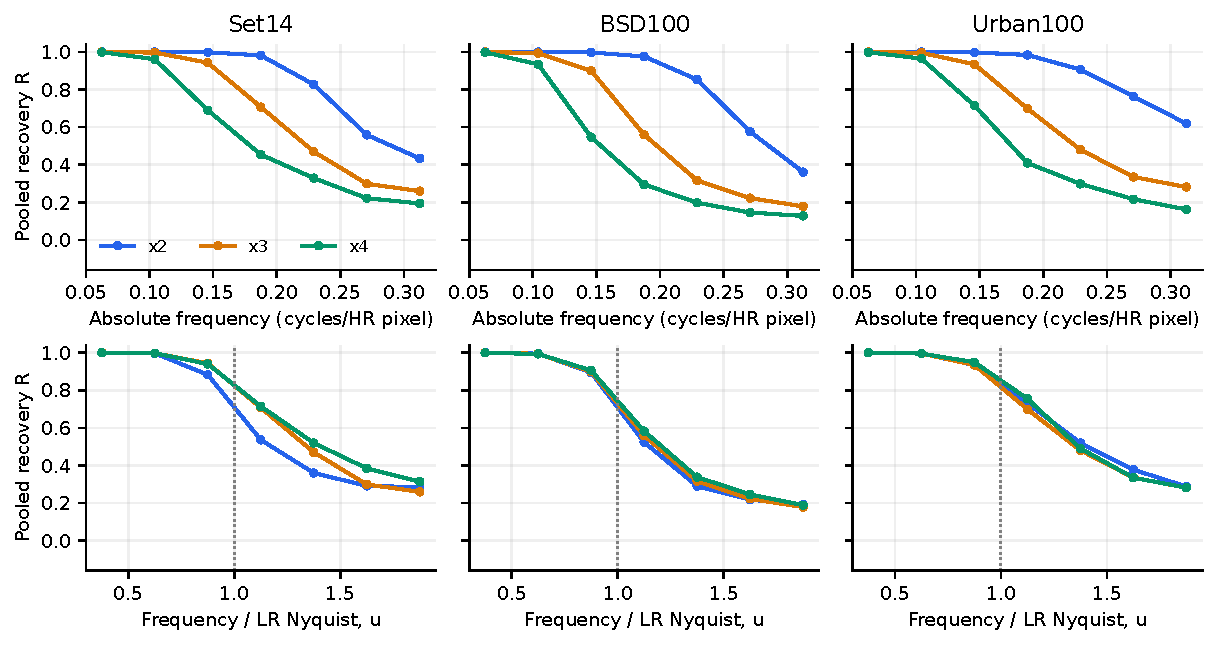
\includegraphics[width=.95\textwidth]{figures/l1-scale-recovery.pdf}
\caption{Scale-dependent recovery of SC-INR (seed1), from the saved L1 energy arrays. Top: fixed absolute-frequency bins. Bottom: the same measurement in LR Nyquist units $u=2s\nu$; the vertical line marks $u=1$. Curves use pooled energy ratios, not a mean of image-wise recoveries. The axes describe evaluated error and need not stay in $[0,1]$. Normalisation substantially reduces scale differences; Table~\ref{tab:l1-main} retains the Set14 threshold failure and all three-model results.}\label{fig:l1-main}
\end{figure*}

\paragraph{Content sensitivity.} A post-hoc leave-one-image-out check identifies barbara as the largest contributor to the Set14 discrepancy. Removing it reduces $D_{\rm in}$ to $.0361/.0298/.0300$ for LIIF/LTE/SC. For comparison, 200 fixed-seed samples of 14 images from the first 30 BSD100 images have respective maxima $.0392/.0378/.0388$. This diagnoses sensitivity of energy pooling to image content; it does not establish JPEG artefacts or a capacity mechanism. We retain the original failed cohort and criterion. Extrapolation and public-model checks likewise remain limited: the original outside-training-range criterion and public-model aggregate each pass only six of nine groups.

\subsection{Paired readout losses and coarse band ordering}\label{sec:readout-main}
The readout comparisons pair LTE with LTE-NoCell and SC-INR with SC-INR-NoSinc under the recovered matched training setup. Define
\begin{equation}\label{eq:loss}
L_b=R_b^{\rm full}-R_b^{\rm ablated}.
\end{equation}
Positive $L_b$ means the full readout improves recovery; negative values are retained. A paired training ablation measures the change between trained models, not the effect of deleting a component while holding all learnt weights fixed. LTE phase conditioning and SC sinc feature modulation are evaluated separately; neither is assumed to implement the same physical pixel integral.

The original F1 small-mismatch predictor $g(R)=R(1-R)^2$ fails the $.5$ correlation threshold for both architectures: $.411/.400$ with linear recovery, $.490/.492$ with network recovery. Cross-architecture loss ranking is high ($.985$), but magnitudes differ. For the correct SC pair, mean losses over $b_1/b_2/b_3$ are $-.0000142/+.0001368/+.0080551$; A-labelled cells average $-.0006091$, and $\times3$ $b_2$ averages $+.0010338$ (LTE: $+.0050$). Some SC cells improve after ablation, including Set14 $\times2$ $b_3$ ($-.03788$). High rank correlation therefore does not imply equal benefits or a common quantitative mechanism.

G1 tests a simpler predictor: the box-footprint versus point-sampling quantity $\epsilon(\nu)=1-\operatorname{sinc}(\nu_x)\operatorname{sinc}(\nu_y)$ gives fixed squared-band scores $(.00006,.00552,.07235)$. It was proposed after seed1 and frozen before seed2/3 evaluation. The full original protocol has been recovered and hash-verified. Table~\ref{tab:g1-main} reports all four confirmatory groups.

\begin{table}[t]\centering\small
\caption{G1: 27 cells per group. Average ranks handle the predictor's three tied band values. Adding $h(R)=R(1-2R)^2$ reduces correlation in every group.}\label{tab:g1-main}
\begin{tabular}{lccc}\toprule
Group & $\rho(\epsilon_b^2,L)$ & $\rho(\epsilon_b^2h(R),L)$ & $L_3>L_2$\\\midrule
LTE seed2 & .577 & .532 & 8/9\\
SC seed2 & .943 & .703 & 9/9\\
LTE seed3 & .676 & .643 & 8/9\\
SC seed3 & .885 & .804 & 9/9\\\bottomrule
\end{tabular}
\end{table}
The original ordering threshold passes in four of four groups; $L_3>L_2$ occurs in 34/36 settings. The additional recovery factor supplies no improvement under the frozen criterion. Because the three scores are strictly increasing, replacing them by band indices $(1,2,3)$ gives exactly the same average ranks and Spearman correlations. The test therefore supports coarse frequency ordering across these architecture--seed groups, with no advantage over that free baseline. It does not validate a gain-mismatch explanation, nor a precise loss amplitude. Saved pooled statistics and coverage are independently checked; G1 did not save per-image signal/error energy weights, so full independent repooling is unavailable.

\subsection{Scale marginalisation predicts ordering but not the ablated function}\label{sec:l2-main}
L2 asks whether a network without a scale readout behaves like the full model averaged over the training-scale inputs. At fixed coordinates and image features, we average predictions over 31 cell inputs corresponding to $s'\in\{1.0,1.1,\ldots,4.0\}$, obtaining $R_{\rm marg}$. The proposed loss is $L_{\rm pred}=R_{\rm full}-R_{\rm marg}$. The primary test covers the 27 $\times2/3/4$ cells; log-spaced queries and $\times8$ are secondary. The uniform scale average is an operational diagnostic, not a conditional distribution of scale given the LR image. This is a post-training diagnostic using HR truth, not a deployable LR-only rule.

\begin{table}[t]\centering\small
\caption{Complete L2 seed2/3 replication. Ratio is the median $L_{\rm pred}/L$ over $L>.005$. Similarity is the fraction of image--scale pairs where the ablated output is closer to the marginalised than the full output.}\label{tab:l2-main}
\begin{tabular}{lcccc}\toprule
Group & $\rho$ & Ratio & Similarity & $\rho-\rho_\epsilon$\\\midrule
LTE seed2 & .712 & .823 & .770 & +.130\\
SC seed2 & .755 & .581 & .689 & $-.142$\\
LTE seed3 & .954 & .833 & .748 & +.331\\
SC seed3 & .700 & .337 & .653 & $-.173$\\\bottomrule
\end{tabular}
\end{table}
Ordering passes in four groups and the magnitude interval $[.5,2]$ in three. Function similarity never reaches $.8$. Superiority over the simple footprint score by at least $.05$ occurs in two groups, below the required three; both are LTE. The cell-invariant ablation control passes in all four groups with maximum difference zero. Independent reconstruction from per-image signal/error energies reproduces the pooled values. The result supports empirical prediction of ordering, while rejecting function equivalence and a uniformly better account across architectures. G1 and L2 differ in crop, image count and colour aggregation, so their correlations are compared within their own protocols.

\section{Checks and Boundaries Beyond ASISR}\label{sec:boundary}
The following completed experiments constrain interpretation of the ASISR baseline. Their full tables and protocols are supplementary; none supplies a nonlinear readout theorem or an adaptive INR selector.

Classical linear experiments show useful approximate cost ranking but numerical counterexamples and unsuccessful winner selection. The complete prospective G2 cohort chooses the same prior in 36/36 cases, trails frame cross-validation by $.112$ dB and costs 1.76 times as much. It establishes neither target-specific adaptation nor an INR selector. The full checks, original criteria and costs are retained in Appendix~\ref{app:guidance-summary} and the supplementary experiment tables. They constrain interpretation rather than extend the paper's central contribution.

\begin{table*}[t]\centering\small
\caption{Claim hierarchy retained in the baseline. Passing a weaker test does not upgrade a failed stronger one.}\label{tab:claims-main}
\begin{tabular}{p{.28\textwidth}p{.35\textwidth}p{.29\textwidth}}\toprule
Question & Complete evidence & Supported conclusion\\\midrule
Does normalisation reduce scale variation? & L1 improves 9/9; strict tolerance passes 6/9 & Useful normalisation; no universal collapse\\
Can a fixed band score order readout losses? & G1 ranks 4/4; adding recovery factor improves 0/4 & Same ranks as band index; no gain mechanism\\
Does scale averaging reproduce the ablation? & L2 ranking 4/4, magnitude 3/4; similarity 0/4 & Correlational prediction; no function equivalence\\
Is L2 better than the simpler predictor? & Improvement in 2/4, below required 3/4 & No general superiority\\
Does calibrated analysis adapt to each target? & G2 constant choice in 36/36; worse accuracy/cost than CV & Default improvement; no adaptive advantage\\\bottomrule
\end{tabular}
\end{table*}

\paragraph{Exploratory evidence retained separately.} Same-observation linear/FF controls on two already-seen images include reverse rankings. A common 32-image empirical evaluation law selects the same strong static prior; it does not isolate a nonlinear mechanism or demonstrate adaptation. An 8-point Gaussian example and the associated finite-sample confidence-set study concern fresh-draw population risk, not single-image safety; they remain classical illustrative material. EEG supplies only 200 calibration segments, with the 760-segment test archive missing. These results motivate scope restrictions rather than cross-modal or new-theory contributions.
